% Sandia National Laboratories is a multimission laboratory managed and
% operated by National Technology & Engineering Solutions of Sandia, LLC, a
% wholly owned subsidiary of Honeywell International Inc., for the U.S.
% Department of Energy’s National Nuclear Security Administration under
% contract DE-NA0003525.

% Copyright 2002-2021 National Technology & Engineering Solutions of Sandia,
% LLC (NTESS).

 
The Power Grid devices are a family of device models that can be used to model  
steady-state power flow in electric power grids.  They include device models for 
branches, bus shunts, transformers and generator buses.  

Power flow in electric power grids can be modeled as a complex-valued voltage-current
problem with standard admittance-matrix techinques. This approach solves the system of
equations $I=YV$, and is termed \texttt{IV} format in this document.  However, it is 
more typically modeled as a power-flow problem that solves the system of equations 
$S = P + jQ = VI^{*}$, where $S$ is the complex power flow, $V$ and $I$ are complex-valued 
quantities, and $I^{*}$ is the complex conjugate of $I$.  The complex power flow can
then be solved in either rectangular or polar coordinates.  These two solution formats are
termed PQ Rectangular (aka, \texttt{PQR} format) and PQ Polar (aka, \texttt{PQP} format) in 
this document.  The variables for each solution format are described in more detail in the
device descriptions given below. 

In all three formulations,an Equivalent Real Formulation (ERF) \cite{Munankarmy} must be used
for compatibility with the existing solver libraries in \Xyce{}.  More details on these 
equations are given below after the individual device descriptions.
 
%%
%% PowerGridBranch Description 
%%
\paragraph{PowerGridBranch}

\begin{Device}\label{PowerGridBranch}

\device
\begin{alltt}
Y<type> <name> <input node1> <output node1> 
+ <input node2> <output node2> [device parameters] 
\end{alltt}
  
\examples
\begin{alltt}
YPowerGridBranch pg1_2 VR1 VR2 VI1 VI2 AT=IV R=0.05 B=0.1 X=0.05
YPGBR pg1_2a VR1 VR2 VI1 VI2 AT=IV R=0.05 B=0.1 X=0.05
YPowerGridBranch pg1_2b VR1 VR2 VI1 VI2 AT=PQR R=0.05 B=0.1 X=0.05
YPGBR pg1_2c VR1 VR2 VI1 VI2 AT=PQR R=0.05 B=0.1 X=0.05
YPowerGridBranch pg1_2d Th1 Th2 VM1 VM2 AT=PQP R=0.05 B=0.1 X=0.05
YPGBR pg1_2e Th1 Th2 VM1 VM2 AT=PQP R=0.05 B=0.1 X=0.05
\end{alltt}

\parameters 
\begin{Parameters}
\param{type}
The device type has a verbose (\texttt{PowerBranchBranch}) and a shortened
(\texttt{PGBR}) form.  Their usage may be mixed within a netlist.

\param{name}
Name of the device instance. This must be present, and unique amongst the 
\texttt{PowerGridBranch} devices in the netlist.

\param{input node}
There are two input nodes, \texttt{<input node1>} and \texttt{<input node2>}, 
whose definitions depend on the AnalysisType (\texttt{AT}) specified.  Both nodes
must be specified.  This device can be viewed as a generalized 4-port resistor, using
the Equivalent Real Form (ERF) described below in the equation subsections. For 
\texttt{IV} and \texttt{PQR} formats, \texttt{<input node1>} is the real part 
(\texttt{VR}) of the voltage at terminal 1 while \texttt{<input node2>} is the 
imaginary part (\texttt{VI}) of the voltage at terminal 1.  
For \texttt{PQP} format, \texttt{<input node1>} is the angle ($\Theta$ or \texttt{Th}) of the voltage 
at terminal 1 while \texttt{<input node2>} is the magnitude (\texttt{VM} or $|V|$) of the 
voltage at terminal 1.  Finally, by analogy to other \Xyce{} devices, node 1 can be 
considered as the positive terminal for this device, while node 2 is the negative
terminal.

\param{output node}
There are two output nodes, \texttt{<output node1>} and \texttt{<output node2>}, 
whose definitions depend on the AnalysisType (\texttt{AT}) specified.  Both nodes
must be specified.  This device can be viewed as a generalized 4-port resistor, 
using the ERF described below in the equation subsections. For \texttt{IV} 
and \texttt{PQR} formats, \texttt{<output node1>} is the real part (\texttt{VR}) of 
the voltage at terminal 2 while \texttt{<output node2>} is the imaginary part 
(\texttt{VI}) of the voltage at terminal 2.  
For \texttt{PQP} format, \texttt{<output node1>} is the angle ($\Theta$ or \texttt{Th}) of the voltage 
at terminal 2 while \texttt{<output node2>} is the magnitude (\texttt{VM} or $|V|$) of the 
voltage at terminal 2.  Finally, by analogy to other \Xyce{} devices, node 2 can be 
considered as the negative terminal for this device, while node 1 is the positive
terminal.

\param{AT}
This device supports all three analysis types (\texttt{AT}), namely \texttt{IV}, 
\texttt{PQR} and \texttt{PQP}.  The equations for these analysis types are described 
below.  All power grid devices, of all types, in a \Xyce{} netlist must use the 
same analysis type.  This constraint is not checked during netlist parsing.  
Violation of this constraint may cause unpredictable results.

\param{B}
Branch susceptance, given in per unit.  As discussed in the Equation section below, 
the susceptance value given on the branch description lines in 
IEEE Common Data Format (CDF) files is split equally between terminals 1 and 2.

\param{R} 
Branch resistance, given in per unit.

\param{X}
Branch reactance, given in per unit.

\end{Parameters}
\end{Device}

\paragraph{PowerGridBranch Device Parameters}

%%
%% PowerGridBusBranch Instance Parameter Table
%%
% This table was generated by Xyce:
%   Xyce -doc PowerGridBranch 1
%
\index{powergridbranch!device instance parameters}
\begin{DeviceParamTableGenerated}{PowerGridBranch Device Instance Parameters}{PowerGridBranch_1_Device_Instance_Params}
AT & Analysis Type & -- & 'PQP' \\ \hline
B & Branch Shunt Susceptance & per unit & 0 \\ \hline
R & Branch Resistance & per unit & 0 \\ \hline
X & Branch Reactance & per unit & 0 \\ \hline
\end{DeviceParamTableGenerated}



%%
%% PowerGridBusShunt Description
%%
\paragraph{PowerGridBusShunt}

\begin{Device}\label{PowerGridBusShunt}

\device
\begin{alltt}
Y<type> <name> <input node1> <output node1> 
+ <input node2> <output node2 [device parameters] 
\end{alltt}
  
\examples
\begin{alltt}
YPowerGridBusShunt pg1_2 VR1 VR2 VI1 VI2 AT=IV R=0.05 B=0.1 X=0.05
YPGBS pg1_2a VR1 VR2 VI1 VI2 AT=IV R=0.05 B=0.1 X=0.05
YPowerGridBusShunt pg1_2b VR1 VR2 VI1 VI2 AT=PQR R=0.05 B=0.1 X=0.05
YPGBS pg1_2c VR1 VR2 VI1 VI2 AT=PQR R=0.05 B=0.1 X=0.05
YPowerGridBusShunt pg1_2d Th1 Th2 VM1 VM2 AT=PQP R=0.05 B=0.1 X=0.05
YPGBS pg1_2e Th1 Th2 VM1 VM2 AT=PQP R=0.05 B=0.1 X=0.0
\end{alltt}

\parameters 
\begin{Parameters}
\param{type}
The device type has a verbose (\texttt{PowerGridBusShunt}) and a shortened
(\texttt{PGBS}) form.  Their usage may be mixed within a netlist.

\param{name}
Name of the device instance.  This must be present, and unique amongst the 
\texttt{PowerGridBusShunt} devices in the netlist.

\param{input node}
There are two input nodes, \texttt{<input node1>} and \texttt{<input node2>}, 
whose definitions depend on the AnalysisType (\texttt{AT}) specified.  Both nodes
must be specified.  This device can be viewed as a generalized 4-port resistor, using
the Equivalent Real Form (ERF) described below in the equation subsections. For 
\texttt{IV} and \texttt{PQR} formats, \texttt{<input node1>} is the real part 
(\texttt{VR}) of the voltage at terminal 1 while \texttt{<input node2>} is the 
imaginary part (\texttt{VI}) of the voltage at terminal 1.  
For \texttt{PQP} format, \texttt{<input node1>} is the angle ($\Theta$ or \texttt{Th}) of the voltage 
at terminal 1 while \texttt{<input node2>} is the magnitude (\texttt{VM} or $|V|$) of the 
voltage at terminal 1.  Finally, by analogy to other \Xyce{} devices, node 1 can be 
considered as the positive terminal for this device, while node 2 is the negative
terminal.

\param{output node}
There are two output nodes, \texttt{<output node1>} and \texttt{<output node2>}, 
whose definitions depend on the AnalysisType (\texttt{AT}) specified.  Both nodes
must be specified.  This device can be viewed as a generalized 4-port resistor, 
using the ERF described below in the equation subsections. For \texttt{IV} 
and \texttt{PQR} formats, \texttt{<output node1>} is the real part (\texttt{VR}) of 
the voltage at terminal 2 while \texttt{<output node2>} is the imaginary part 
(\texttt{VI}) of the voltage at terminal 2.  
For \texttt{PQP} format, \texttt{<output node1>} is the angle ($\Theta$ or \texttt{Th}) of the voltage 
at terminal 2 while \texttt{<output node2>} is the magnitude (\texttt{VM} or $|V|$) of the 
voltage at terminal 2.  Finally, by analogy to other \Xyce{} devices, node 2 can be 
considered as the negative terminal for this device, while node 1 is the positive
terminal.
  
\param{AT}
This device supports all three analysis types (\texttt{AT}), namely \texttt{IV}, 
\texttt{PQR} and \texttt{PQP}.  The equations for these analysis types are described 
below.  All power grid devices, of all types, in a \Xyce{} netlist must use the same
analysis type.  This constraint is not checked during netlist parsing.  Violation of 
this constraint may cause unpredictable results.

\param{B}
Shunt susceptance, given in per unit.

\param{G}
Shunt conductance, given in per unit.

\end{Parameters}
\end{Device}

\paragraph{Bus Shunt Device Parameters}

%%
%% PowerGridBusShunt Table
%%
% This table was generated by Xyce:
%   Xyce -doc PowerGridBusShunt 1
%
\index{powergridbusshunt!device instance parameters}
\begin{DeviceParamTableGenerated}{PowerGridBusShunt Device Instance Parameters}{PowerGridBusShunt_1_Device_Instance_Params}
AT & Analysis Type & -- & 'PQP' \\ \hline
B & Shunt Susceptance & per unit & 0 \\ \hline
G & Shunt Conductance & per unit & 0 \\ \hline
\end{DeviceParamTableGenerated}



%%
%% PowerGridTransformer Description
%%
\paragraph{PowerGridTransformer}

\begin{Device}\label{PowerGridTransformer}

\device
\begin{alltt}
Y<type> <name> <input node1> <output node1> 
+ <input node2> <output node2> [control node] [device parameters] 
\end{alltt}
  
\examples
\begin{alltt}
YPowerGridTransformer pg1_2 VR1 VR2 VI1 VI2 AT=IV R=0.05 X=0.05 
+ TR=0.9 PS=0.1
YPGTR pg1_2a VR1 VR2 VI1 VI2 AT=IV R=0.05 X=0.05 TR=0.9 PS=\{18*PI/180\}
YPowerGridTransformer pg1_2b VR1 VR2 VI1 VI2 AT=PQR R=0.05 X=0.05 
+ TR=0.9 PS=0.1
YPGTR pg1_2c VR1 VR2 VI1 VI2 AT=PQR R=0.05 B=0.1 X=0.05 TR=0.9 PS=0.1
YPowerGridTransformer pg1_2d Th1 Th2 VM1 VM2 AT=PQP 
+ R=0.05 X=0.05 PS=\{18*PI/180\}
YPGTR pg1_2e Th1 Th2 VM1 VM2 AT=PQP R=0.05 X=0.0 TR=0.9 PS=0.1
YPGTR pg1_2f Th1 Th2 VM1 VM2 N AT=PQP R=0.05 X=0.0 TT=VT PS=0.1
YPGTR pg1_2g Th1 Th2 VM1 VM2 Phi AT=PQP R=0.05 X=0.0 TT=PS TR=0.9
\end{alltt}

\parameters 
\begin{Parameters}
\param{type}
The device type has a verbose (\texttt{PowerGridTransformer}) and a shortened
(\texttt{PGTR}) form.  Their usage may be mixed within a netlist.

\param{name}
Name of the device instance.  This must be present, and unique amongst the 
\texttt{PowerGridTransformer} devices in the netlist.

\param{input node}
There are two input nodes, \texttt{<input node1>} and \texttt{<input node2>}, 
whose definitions depend on the AnalysisType (\texttt{AT}) specified.  Both nodes
must be specified.  This device can be viewed as a generalized 4-port resistor, using
the Equivalent Real Form (ERF) described below in the equation subsections. For 
\texttt{IV} and \texttt{PQR} formats, \texttt{<input node1>} is the real part 
(\texttt{VR}) of the voltage at terminal 1 while \texttt{<input node2>} is the 
imaginary part (\texttt{VI}) of the voltage at terminal 1.  
For \texttt{PQP} format, \texttt{<input node1>} is the angle ($\Theta$ or \texttt{Th}) of the voltage 
at terminal 1 while \texttt{<input node2>} is the magnitude (\texttt{VM} or $|V|$) of the 
voltage at terminal 1.  Finally, by analogy to other \Xyce{} devices, node 1 can be 
considered as the positive terminal for this device, while node 2 is the negative
terminal.

\param{output node}
There are two output nodes, \texttt{<output node1>} and \texttt{<output node2>}, 
whose definitions depend on the AnalysisType (\texttt{AT}) specified.  Both nodes
must be specified.  This device can be viewed as a generalized 4-port resistor, 
using the ERF described below in the equation subsections. For \texttt{IV} 
and \texttt{PQR} formats, \texttt{<output node1>} is the real part (\texttt{VR}) of 
the voltage at terminal 2 while \texttt{<output node2>} is the imaginary part 
(\texttt{VI}) of the voltage at terminal 2.  
For \texttt{PQP} format, \texttt{<output node1>} is the angle ($\Theta$ or \texttt{Th}) of the voltage 
at terminal 2 while \texttt{<output node2>} is the magnitude (\texttt{VM} or $|V|$) of the 
voltage at terminal 2.  Finally, by analogy to other \Xyce{} devices, node 2 can be 
considered as the negative terminal for this device, while node 1 is the positive
terminal.

\param{control input}
This is an optional node.  However, it must be specified on the instance line if the 
transformer type (\texttt{TT}) is set to either 2 or 3.  It does not exist, and must 
not be specified on the instance line, for the default of \texttt{TT}=1.  The use of 
the \texttt{control input} node is covered under the definition of the \texttt{TT} 
instance parameter.

\param{AT}
This device supports all three analysis types (\texttt{AT}), namely \texttt{IV}, 
\texttt{PQR} and \texttt{PQP}.  The equations for these analysis types are described 
below.  All power grid devices, of all types, in a \Xyce{} netlist must use the same 
analysis type.  This constraint is not checked during netlist parsing.  Violation of 
this constraint may cause unpredictable results.

\param{PS}
Phase shift given in radians.  As illustrated above, \texttt{PS=\{18*PI/180\}} is a
convenient syntax for converting between decimal degrees and radians on a \Xyce{}
instance line.  This instance parameter is ignored if \texttt{TT}=3, since the
phase shift is set by the optional \texttt{control node} in that case.

\param{R}
Resistance, given in per unit.

\param{TR}
Turns ratio, given in per unit.  This instance parameter is ignored if \texttt{TT}=2,
since this value is set by the optional \texttt{control node} in that case..

\param{X}
Reactance, given in per unit.

\param{TT}
This is the ``Transformer Type''. It allows the user to implement tap-changing
or phase-shifting transformers, by attaching an appropriate control-circuit to the 
\texttt{control input} node.  The allowed values for \texttt{TT} are \texttt{FT}, 
\texttt{VT} or \texttt{PS}, with default value of \texttt{FT}.  Any other values
will cause a netlist parsing error.  A transformer type of \texttt{FT} has a 
fixed turns-ratio, and is a four-terminal device with
two input nodes (\texttt{<input node1>} and \texttt{<input node2>}) and two output
nodes (\texttt{<output node1>} and \texttt{<output node2>}). Let the effective complex 
turns ratio be $r = m + jp = n*(cos(\phi) + j*sin(\phi))$.  The transformer type of
\texttt{VT} exposes the $n$ variable as the \texttt{control input} node, and hence can
operate with a variable turns-ratio. The  transformer type of \texttt{PS} exposes the 
$\phi$ variable as the \texttt{control input} node, and hence can act as a phase shifter. 
The instantaneous value of $n$ (or $\phi$) can be set to the voltage applied to the 
\texttt{control input} node.  There will be no current draw into (or out of) the
\texttt{control input} node.  This device model does not yet support simultaneously
varying both $n$ and $\phi$.
\end{Parameters}
\end{Device}

\paragraph{Transformer Device Parameters}

%%
%% PowerGridTransformer Device Instance Parameter Table
%%
% This table was generated by Xyce:
%   Xyce -doc PowerGridTransformer 1
%
\index{powergridtransformer!device instance parameters}
\begin{DeviceParamTableGenerated}{PowerGridTransformer Device Instance Parameters}{PowerGridTransformer_1_Device_Instance_Params}
AT & Analysis Type & -- & 'PQP' \\ \hline
PS & Phase Shift & rad & 0 \\ \hline
R & Resistance & per unit & 0 \\ \hline
TR & Transformer Turns Ratio & per unit & 1 \\ \hline
TT & Transformer Type & -- & 'FT' \\ \hline
X & Reactance & per unit & 0 \\ \hline
\end{DeviceParamTableGenerated}



%%
%% PowerGridGenBus Description
%%
\paragraph{PowerGridGenBus}

\begin{Device}\label{PowerGridGenBus}

\device
\begin{alltt}
Y<type> <name> <input node1> <output node1> 
+ <input node2> <output node2> [device parameters] 
\end{alltt}
  
\examples
\begin{alltt}
YPowerGridGenBus GenBus1 Th1 0 VM1 0 AT=PQP VM=1.045 P=0.4
YPGGB GenBus2 Th2 GND VM2 GND AT=PQP VM=1.045 P=0.4
\end{alltt}

\parameters 
\begin{Parameters}
\param{type}
The device type has a verbose (\texttt{PowerGridGenBus}) and a shortened
(\texttt{PGGB}) form.  Their usage may be mixed within a netlist.

\param{name}
Name of the device instance.  This must be present, and unique amongst the 
\texttt{PowerGridGenBus} devices in the netlist.

\param{input node}
There are two input nodes, \texttt{<input node1>} and \texttt{<input node2>}, 
whose definitions depend on the AnalysisType (\texttt{AT}) specified.  Both nodes
must be specified.  This device can be viewed as a generalized 4-port resistor, using
the Equivalent Real Form (ERF) described below in the equation subsections. For 
\texttt{IV} and \texttt{PQR} formats, \texttt{<input node1>} is the real part 
(\texttt{VR}) of the voltage at terminal 1 while \texttt{<input node2>} is the 
imaginary part (\texttt{VI}) of the voltage at terminal 1.  
For \texttt{PQP} format, \texttt{<input node1>} is the angle ($\Theta$ or \texttt{Th}) of the voltage 
at terminal 1 while \texttt{<input node2>} is the magnitude (\texttt{VM} or $|V|$) of the 
voltage at terminal 1.  Finally, by analogy to other \Xyce{} devices, node 1 can be 
considered as the positive terminal for this device, while node 2 is the negative
terminal.

\param{output node}
There are two output nodes, \texttt{<output node1>} and \texttt{<output node2>}, 
whose definitions depend on the AnalysisType (\texttt{AT}) specified.  Both nodes
must be specified.  This device can be viewed as a generalized 4-port resistor, 
using the ERF described below in the equation subsections. For \texttt{IV} 
and \texttt{PQR} formats, \texttt{<output node1>} is the real part (\texttt{VR}) of 
the voltage at terminal 2 while \texttt{<output node2>} is the imaginary part 
(\texttt{VI}) of the voltage at terminal 2.  
For \texttt{PQP} format, \texttt{<output node1>} is the angle ($\Theta$ or \texttt{Th}) of the voltage 
at terminal 2 while \texttt{<output node2>} is the magnitude (\texttt{VM} or $|V|$) of the 
voltage at terminal 2.  Finally, by analogy to other \Xyce{} devices, node 2 can be 
considered as the negative terminal for this device, while node 1 is the positive
terminal.

\param{AT}
This device currently only supports the \texttt{PQP} analysis type (\texttt{AT}). 
The equations for the  \texttt{PQP} analysis type are described below.  All power grid
devices, of all types, in a \Xyce{} netlist must use the same analysis type.  This 
constraint is not checked during netlist parsing.  Violation of this constraint may 
cause unpredictable results.

\param{P} 
Generator Output Power, given in per unit.  As noted below, positive real power
(\texttt{P}) and positive reactive power (\texttt{Q}) flow out of the positive 
(\texttt{<input node1>} and \texttt{<input node2>}) terminals into the power grid.
This is opposite from the normal convention for voltage and current sources
in \Xyce{} and SPICE. 

\param{QLED}
This is the Q-Limit Enforcement Delay.  It is only used if either \texttt{QMAX} or
\texttt{QMIN} is specified.  The Q-Limits are not enforced for the first \texttt{QLED}
Newton iterations of the DC Operating Point (DCOP) calculation.  This may be useful if
a given generator bus has, for example, a very small value of \texttt{QMIN} ~\cite{Milano}.
If \texttt{QMAX} or \texttt{QMIN} is specified and \texttt{QLED} is omitted then the default
\texttt{QLED} value of 0 is used.

\param{QMAX}
The upper limit on the reactive power (\texttt{Q}) flow into the power grid, given in per unit.
If this parameter is omitted on the instance line then no upper limit on the reactive power flow
is enforced.  It is recommended that either both \texttt{QMAX} and \texttt{QMIN} be
specified or that both be omitted.

\param{QMIN}
The lower limit on the reactive power (\texttt{Q}) flow into the power grid, given in per unit. 
If this parameter is omitted on the instance line then no lower limit on the reactive power flow
is enforced.  It is recommended that either both \texttt{QMAX} and \texttt{QMIN} be
specified or that both be omitted. 

\param{VM}
Fixed voltage magnitude, given in per unit.

\end{Parameters}
\end{Device}

\paragraph{Generator Bus Device Parameters}

%%
%% PowerGridGenBus Table
%%
% This table was generated by Xyce:
%   Xyce -doc PowerGridGenBus 1
%
\index{powergridgenbus!device instance parameters}
\begin{DeviceParamTableGenerated}{PowerGridGenBus Device Instance Parameters}{PowerGridGenBus_1_Device_Instance_Params}
AT & Analysis Type & -- & 'PQP' \\ \hline
P & Generator Output Power & per unit & 1 \\ \hline
QLED & Q-Limit Enforcement Delay & -- & 0 \\ \hline
QMAX & Reactive Power Max Limit & per unit & 1 \\ \hline
QMIN & Reactive Power Min Limit & per unit & 0 \\ \hline
VM & Voltage Magnitude & per unit & 1 \\ \hline
\end{DeviceParamTableGenerated}


\paragraph{Branch Current and Power Accessors}
This version of the Power Grid devices does not support the branch current accessor, \texttt{I()}, 
or the power accessors, \texttt{P()} or \texttt{W()}.

\paragraph{Compatibility with .STEP}
\texttt{.STEP} should work with all of the instance parameters for the power grid devices. 
The two exceptions are the Analysis Type (\texttt{AT}) for all of the power grid devices 
and the Transformer Type (\texttt{TT}) for the Transformer device.  Those two parameters
must be constant for all steps. 

\paragraph{Model Limitations and Caveats}
The following features are not supported by this release of the Power Grid device models.
\begin{XyceItemize}
  \item The Generator Bus device model only supports the PQ Polar format. So, reactive 
     power (\texttt{QMAX} and \texttt{QMIN}) limits in the Generator Bus device model are
     also only supported for that format.
  \item Magnetizing susceptance for transformers.
  \item Certain instance parameters, or combinations of instance parameters, will cause
     errors during netlist parsing.  In particular, either \texttt{B}, \texttt{R} or 
     \texttt{X} must be non-zero for the Branch device.  Either \texttt{B} or
     \texttt{G} must be non-zero for the Bus Shunt device.  Either \texttt{R} or
     \texttt{X} must be non-zero for the Transformer device.  \texttt{TR} must not
     be zero for the Transformer device.  \texttt{VM} must be positive for the 
     Generator Bus device. 
\end{XyceItemize}

\paragraph{Equivalent Real Form}
An Equivalent Real Form (ERF) must be used to make the complex-valued voltage-current 
and power-flow equations compatible with the real-valued solvers used by \Xyce{}.  The 
equations given below use a K1 ERF ~\cite{Munankarmy}, which 
solves the complex-valued system of equations $I=YV$ as follows.  Let $Y=(g+jb)$, 
$V=(V_{R}+jV_{I})$ and $I=(I_{R}+jI_{I})$.  Then the equivalent set of real-valued equations is:

\begin{equation}
  \left[ \begin{array}{c} I_{R} \\ I_{I}
         \end{array} \right] =
  \left[ \begin{array}{cc} 
         g & -b \\ g & b \\  
         \end{array} \right] 
  \left[ \begin{array}{c} V_{R} \\ V_{I}
          \end{array} \right]
\end{equation}

\paragraph{Y Matrices for Power Grid Branch and Bus Shunt}
The Y-Matrix for the \texttt{PowerGridBranch} device can be expressed as follows where $A=(R+jX)^{-1}$,
$R$ is the branch resistance, $X$ is the branch reactance and $B$ is the branch shunt susceptance given
on the device's instance line:

\begin{equation}
  \left[ \begin{array}{cc} 
         Y_{11} & Y_{12} \\ Y_{21} & Y_{22} \\  
         \end{array} \right] =
  \left[ \begin{array}{cc} 
         g_{11}+jb_{11} & g_{12}+jb_{12} \\  g_{21}+jb_{21} & g_{22}+jb_{22}
         \end{array} \right] =
  \left[ \begin{array}{cc} 
         A & -A+0.5j*B \\ -A+0.5j*B & A
         \end{array} \right]
\end{equation}
% PI-model for PowerGridBranch
\begin{figure}[ht]
  \centering
  \scalebox{1.0}
  {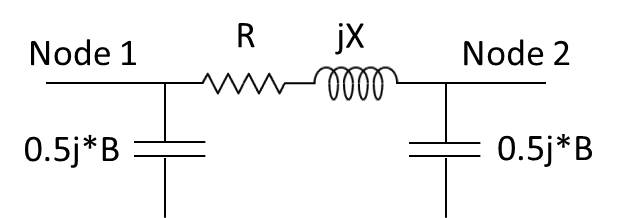
\includegraphics[width=3.2in,height= 1.14in]{PowerGridBranch.jpg}}
  \caption[Lumped $\Pi$ Model for PowerGridBranch]{Lumped $\Pi$ Model for PowerGridBranch. \label{figPowerGridBranch}}
\end{figure}
The Y-Matrix for the \texttt{PowerGridBusShunt} device can be expressed as follows where 
$G$ is the bus shunt conductance and $B$ is the bus shunt susceptance given
on the device's instance line:

\begin{equation}
  \left[ \begin{array}{cc} 
         Y_{11} & Y_{12} \\ Y_{21} & Y_{22} \\  
         \end{array} \right] =
  \left[ \begin{array}{cc} 
         g_{11}+jb_{11} & g_{12}+jb_{12} \\  g_{21}+jb_{21} & g_{22}+jb_{22}
         \end{array} \right] =
  \left[ \begin{array}{cc} 
         G+jB & -G-jB \\ -G-jB & G+jB
         \end{array} \right]
\end{equation}
% Model for PowerGridBusShunt
\begin{figure}[ht]
  \centering
  \scalebox{1.0}
  {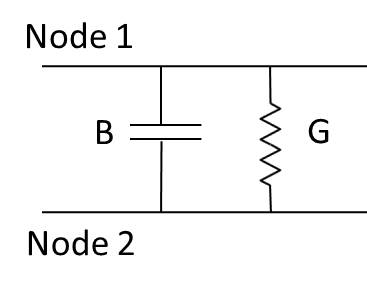
\includegraphics[width=1.91in,height= 1.43in]{PowerGridBusShunt.jpg}}
  \caption[Equivalent Circuit for PowerGridbusShunt]{Equivalent Circuit for PowerGridBusShunt. \label{figPowerGridBusShunt}}
\end{figure}
\paragraph{Equations Common to Power Grid Branch and Bus Shunt}
The \texttt{PowerGridBranch} and \texttt{PowerGridBusShunt} devices use the same
basic equations to model voltage and current flow or voltage and power flow. The 
differences are in the Y-Matrices described above.  There are three options for 
the equations used, namely I=YV, PQ Polar and PQ Rectangular.

For the I=YV format, the device equations for the \texttt{PowerGridBranch} and 
\texttt{PowerGridBusShunt} devices are as follows, where the $g_{ij}$ and $b_{ij}$ 
terms are given above.  Also, $V_{R1}$ and $V_{I1}$ are the real and imaginary parts 
of the voltage at terminal 1.  $I_{R1}$ and $I_{I1}$ are the real and imaginary parts 
of the current at terminal 1.

\begin{equation}
  \left[ \begin{array}{c} I_{R1} \\ I_{R2} \\ I_{I1} \\ I_{I2} 
         \end{array} \right] =
  \left[ \begin{array}{cccc}
      g_{11} & g_{12} & -b_{11} & -b_{12} \\
      g_{21} & g_{22} & -b_{21} & -b_{22} \\
      b_{11} & b_{12} & g_{11} & g_{12} \\
      b_{21} & b_{22} & g_{21} & g_{22} \\
      \end{array} \right] 
  \left[ \begin{array}{c} V_{R1} \\ V_{R2} \\ V_{I1} \\ V_{I2}
         \end{array} \right]
\end{equation}

For the PQ Rectangular format, the device equations are nonlinear ~\cite{Milano}.
\begin{eqnarray}
  P_{1} = g_{11}(V_{R1}^{2} + V_{I1}^{2}) + V_{R1}(g_{12}*V_{R2}-b_{12}*V_{I2})
         + V_{I1}(b_{12}*V_{R2}+g_{12}*V_{I2})\\ 
  P_{2} = g_{22}(V_{R2}^{2} + V_{I2}^{2}) + V_{R2}(g_{21}*V_{R1}-b_{21}*V_{I1})
         + V_{I2}(b_{21}*V_{R1}+g_{21}*V_{I1})\\ 
  Q_{1} = -b_{11}(V_{R1}^{2} + V_{I1}^{2}) + V_{I1}(g_{12}*V_{R2}-b_{12}*V_{I2})
         + V_{R1}(b_{12}*V_{R2}+g_{12}*V_{I2})\\  
  Q_{2} = -b_{22}(V_{R2}^{2} + V_{I2}^{2}) + V_{I2}(g_{21}*V_{R1}-b_{21}*V_{I1})
         + V_{R2}(b_{21}*V_{R1}+g_{21}*V_{I1})
\end{eqnarray}

For the PQ Polar format, the device equations are also nonlinear ~\cite{Milano}. 
Define $|V_{1}|$ as the voltage magnitude at terminal 1 and $\Theta_{1}$ as the 
voltage angle at terminal 1.
\begin{eqnarray}
  P_{1} = g_{11} * |V_{1}|^{2} 
        + |V_{1}| * |V_{2}| * (g_{12}*cos(\Theta_{1}-\Theta_{2}) + b_{12}*sin(\Theta_{1}-\Theta_{2}))\\ 
  P_{2} = g_{22} * |V_{2}|^{2} 
        + |V_{2}| * |V_{1}| * (g_{21}*cos(\Theta_{2}-\Theta_{1}) + b_{21}*sin(\Theta_{2}-\Theta_{1}))\\ 
  Q_{1} =  -b_{11} * |V_{1}|^{2} 
        + |V_{1}| * |V_{2}| * (g_{12}*sin(\Theta_{1}-\Theta_{2}) - b_{12}*cos(\Theta_{1}-\Theta_{2}))\\ 
  Q_{2} =  -b_{22} * |V_{2}|^{2} 
        + |V_{2}| * |V_{1}| * (g_{21}*sin(\Theta_{2}-\Theta_{1}) - b_{21}*cos(\Theta_{2}-\Theta_{1}))
\end{eqnarray}

\paragraph{Equations for Power Grid Transformer}
The equations for the PowerGridTransformer device are similar to those used by the 
PowerGridBranch and PowerGridBusShunt devices.  The circuit diagram for the
PowerGridTransformer is shown below.

For I=YV and PQ Rectangular formats, the equations are the same as for the \texttt{PowerGridBranch}
and \texttt{PowerBusBusShunt} devices.  However, the following Y-Matrix is used where
where $A=(R+jX)^{-1}$, $R$ is the resistance, $X$ is the reactance, $n$ is the turns ratio (which is
the \texttt{TR} instance parameter) and $\phi$ is the phase shift in radians (which is 
the \texttt{PS} instance parameter).

For the I=YV and PQ Rectangular formats, the Y matrix is not symmetric and is given by the following
\cite{Kundur}. Let the effective complex turns ratio be $r = m + jp = n*(cos(\phi) + j*sin(\phi))$:

\begin{equation}
  \left[ \begin{array}{cc} 
         Y_{11} & Y_{12} \\ Y_{21} & Y_{22} \\  
         \end{array} \right] =
  \left[ \begin{array}{cc} 
         g_{11}+jb_{11} & g_{12}+jb_{12} \\  g_{21}+jb_{21} & g_{22}+jb_{22}
         \end{array} \right] =
  \left[ \begin{array}{cc} 
         A*(m^{2}+p^{2})^{-1} & -A*(m-jp)^{-1} \\ -A*(m+jp)^{-1} & A
         \end{array} \right]
\end{equation}

The voltage-current and power flow equations for the I=YV and PQ Rectangular formats
are then the same as for the \texttt{PowerGridBranch}
and \texttt{PowerGridBusShunt} devices, with the modified Y-matrix parameters given above.

For the PQ Polar format, the Y matrix is not symmetric and is given by ~\cite{Milano}:

\begin{equation}
  \left[ \begin{array}{cc} 
         Y_{11} & Y_{12} \\ Y_{21} & Y_{22} \\  
         \end{array} \right] =
  \left[ \begin{array}{cc} 
         g_{11}+jb_{11} & g_{12}+jb_{12} \\  g_{21}+jb_{21} & g_{22}+jb_{22}
         \end{array} \right] =
  \left[ \begin{array}{cc} 
         A*n^{-2} & -A*n^{-1} \\ -A*n^{-1} & A
         \end{array} \right]
\end{equation}
% Model for PowerGridBranch
\begin{figure}[ht]
  \centering
  \scalebox{1.0}
  {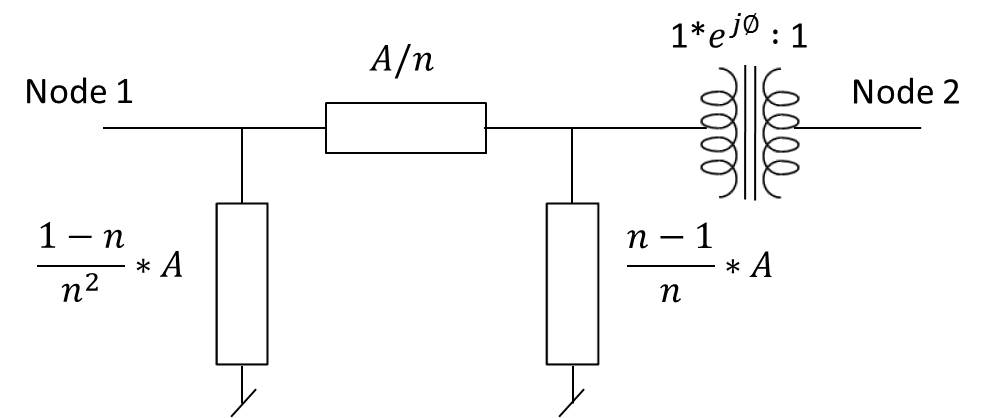
\includegraphics[width=5.17in,height= 2.21in]{PowerGridTransformer.jpg}}
  \caption[Equivalent Circuit for PowerGridTransformer]{Equivalent Circuit for PowerGridTransformer. \label{figPowerGridTransformer}}
\end{figure}
The power flow equation for PQ Polar format are then:
\begin{eqnarray}
  P_{1} = g_{11} * |V_{1}|^{2} 
        + |V_{1}| * |V_{2}| * (g_{12}*cos(\Theta_{1}-\Theta_{2}-\phi) 
                            + b_{12}*sin(\Theta_{1}-\Theta_{2}-\phi))\\ 
  P_{2} = g_{22} * |V_{2}|^{2} 
        + |V_{2}| * |V_{1}| * (g_{21}*cos(\Theta_{2}-\Theta_{1}+\phi) 
                            + b_{21}*sin(\Theta_{2}-\Theta_{1}+\phi))\\ 
  Q_{1} =  -b_{11} * |V_{1}|^{2} 
        + |V_{1}| * |V_{2}| * (g_{12}*sin(\Theta_{1}-\Theta_{2}-\phi) 
                            - b_{12}*cos(\Theta_{1}-\Theta_{2}-\phi))\\ 
  Q_{2} =  -b_{22} * |V_{2}|^{2} 
        + |V_{2}| * |V_{1}| * (g_{21}*sin(\Theta_{2}-\Theta_{1}+\phi) 
                             - b_{21}*cos(\Theta_{2}-\Theta_{1}+\phi))
\end{eqnarray}

\paragraph{Equations for Power Grid Gen Bus}
The \texttt{PowerGridGenBus} is an active device that functions as an ideal generator 
with a fixed power output ($P$) and voltage magnitude ($VM$).  Reactive power 
(\texttt{QMAX} and \texttt{QMIN}) limits are also supported.  The device equations
for the PQ Polar format are as follows ~\cite{Milano}.  The other solution formulations are 
not supported in this release.  If reactive power limits are not being enforced then:
\begin{eqnarray}
P_{1} = P \\|V_{1}| = VM
\end{eqnarray}
If reactive power limits are being enforced then $P_{1}$ is still held constant but the behavior
of the $V_{1}$ terminal changes between a constant-voltage and a constant-current source.
In particular, $|V_{1}| = VM$ only if \texttt{QMIN} $< Q_{1} <$ \texttt{QMAX}.  Otherwise, 
$|V_{1}|$ is unconstrained and the appropriate \texttt{QMIN} or \texttt{QMAX} value is 
enforced at the $V_{1}$ terminal instead.

The convention for Power Grids is that positive power is injected into the grid.
So, positive real (P) and reactive power (Q) flow out of the positive terminals 
(\texttt{inputNode 1} and \texttt{inputNode 2}).  This is reversed from the normal
convention for current direction for voltage and current sources in either \Xyce{} 
or SPICE.
